\documentclass[a4paper,10pt]{article}
\usepackage[utf8]{inputenc}
\usepackage{graphicx}
\usepackage{url}
\usepackage{float}
\usepackage{times}
\usepackage{multirow}
\usepackage{listings}
\usepackage{times}
\usepackage{paralist}
\usepackage{epsfig}
\usepackage[figtopcap]{subfigure}
\usepackage[hypertex]{hyperref}
\usepackage{subfigure}
\usepackage{color}



%\documentclass{rspublic}

\usepackage{ifpdf}

\newif\ifdraft
\drafttrue
\ifdraft
\newcommand{\jhanote}[1]{ {\textcolor{red} { ***shantenu: #1 }}}
\newcommand{\alnote}[1]{ {\textcolor{blue} { ***andre: #1 }}}
\newcommand{\athotanote}[1]{ {\textcolor{green} { ***athota: #1 }}}
\else
\newcommand{\alnote}[1]{}
\newcommand{\jhanote}[1]{}
\newcommand{\athotanote}[1]{}
\fi

\newcommand{\I}[1]{\textit{#1}}
\newcommand{\B}[1]{\textbf{#1}}
\newcommand{\BI}[1]{\textbf{\textit{#1}}}
\newcommand{\T}[1]{\texttt{#1}}

\setlength\topmargin{0in}
\setlength\headheight{0in}
\setlength\headsep{0in}
\setlength\textheight{9in}
\setlength\textwidth{6.5in}
\setlength\oddsidemargin{0in}
\setlength\evensidemargin{0in}
\setlength\parindent{0.1in}
\setlength\parskip{0.25em}


\ifpdf
  \DeclareGraphicsExtensions{.pdf, .jpg}
 \else
  \DeclareGraphicsExtensions{.eps, .ps}
\fi

\newcommand{\note}[1]{ {\textcolor{red} { ***NOTE: #1 }}}

\begin{document}
\title{\LARGE Efficient Replica-Exchange Simulations on
  Large-Scale Production Infrastructure}

%Running Asynchronous Replica-Exchange Simulations Across Heterogeneous Distributed Infrastructures}
 
\author{Abhinav Thota$^{1,2}$, Andre Luckow$^{1}$, Shantenu Jha$^{1,2,3}$\\
   \small{\emph{$^{1}$Center for Computation \& Technology, Louisiana State University, USA}}\\
   \small{\emph{$^{2}$Department of Computer Science, Louisiana State University, USA}}\\
   \small{\emph{$^{3}$e-Science Institute, University of Edinburgh, UK}}
   }
 
\maketitle

\section{Introduction}
 
Developing applications that are able to orchestrate heterogeneous
resources across distributed resources is a complex task.  Inevitably,
the design and development of an application is influenced and
constrained by the programming systems and the infrastructure it is
developed against. Breaking this coupling between the development and
the underlying infrastructure, to enable applications to be flexible
(across infrastructure), extensible (to new methods of communication
and coordination) and scalable is an important design objective of
distributed applications -- both logically distributed and physically
distributed.

In this work, we focus on the Replica-Exchange (RE)~\cite{hansmann,Sugita:1999rm} 
methods -- which represent a class of
algorithms that involve a large number of loosely-coupled ensembles.
RE simulations are used to understand physical phenomena -- ranging
from protein folding dynamics to binding affinity calculations.
We develop a flexible, extensible and scalable
implementation of RE that can utilise a range of infrastructure
concurrently (and autonomically/adaptively), that supports different
coordination mechanisms (publish-subscribe, centralised notification),
different replica pairing mechanisms (synchronous versus asynchronous)
and thereby different variants of the RE algorithm. We implement and
demonstrate how a flexible and robust implementation enables the
efficient use of a broad range of infrastructure.

% Several classes of applications, which are well suited for loosely
% coupled Grids, exist; that belongs to this category are
% \emph{Replica Exchange (RE)} simulations.  1 para intro to
% replica-exchange, and how it is traditionally done (ie case I)

\section{Replica-Exchange Approach}

The RE algorithm involves the concurrent execution of multiple similar
simulations, the \emph{replicas}.  There is a loose-coupling between
the replicas in form of periodic exchange attempts between paired
replicas. %Previously, we demonstrated the usage of the SAGA Pilot-Job framework~\cite{saga_bigjob_condor_cloud} -- called the BigJob, to run RE simulations across multiple, heterogeneous distributed Grid and Cloud infrastructures~\cite{Luckow:2008fp}.
%\alnote{maybe we should also intro SAGA at some point} \jhanote{Yes} The Simple API for Grid Applications (SAGA)~\cite{saga_gfd90} is an API standardization effort within the Open Grid Forum (OGF)~\cite{ogf_web}, an international standards development body concerned primarily with standards for distributed computing. The various tasks that are carried out using the SAGA APIs include file staging, job spawning and the conduction of the exchange attempts.
%Further, we introduced several adaptivity modes, e.\,g.\ adaptive
%sampling that are able to react to dynamic changes in resource
%availabilities.

%\alnote{Not sure how many technical we need to provide...}  

%Traditionally, depending
%on the number of processes \texttt{N}, the manager creates \texttt{N/2} pairs
%of replicas.  Before launching a job, the manager ensures that all
%required input files are transferred to the respective resource. For
%this purpose, the SAGA File API and the GridFTP adaptor are used. The
%replica jobs are then submitted to the resource using the SAGA CPR
%API and the MIGOL/GRAM middleware.
\subsection{Traditional Replica Exchange}
For the vanilla implementation of RE (Case I), depending
on the number of processes \texttt{N}, the manager creates \texttt{N/2} pairs
of replicas. When the replicas reach a
pre-determined state (e.g. the NAMD job finishes after a fixed number
of steps), a decision as to whether to exchange temperatures between
previously paired replicas is determined using the Metropolis scheme.
The run of an ensemble of replicas in parallel and the subsequent
pairwise exchange attempt are referred to as generation. No two
replicas can belong to different generations. If the exchange attempt
is successful, parameters such as the temperature are swapped. Both
jobs are then relaunched. % \athotanote{I have tried to put here how
  %the adaptive repex was done, supposing that it was case 1. Or should
 % a general explanation of a replica exchange be here?} \jhanote{I
  %think this is ok}
 
% 1 para limitation on traditional replica exchange
A major limitation of this model is that the replicas are paired in fixed groups. 
Exchanges can only take place between these paired replicas.
This, while limiting the number of replicas which are available for an exchange, also inhibits exchanges between replicas with non-nearest temperatures.% Replicas commonly have to wait for their partners even if another replicas would be available for an exchange. 
This also negates the possibility of crosswalks. A crosswalk is said to occur when a replica originally with a low temperature reaches the upper temperature range and then returns to the lower temperature range. %Moreover, the replicas are attached to their partners, 
%sometimes waiting for them to complete while there are possibly other replicas available which are paired to their partners.
%This also reduces the number of exchanges that can take place within a given time.
Replica pairing works well in an ideal scenario but with heterogeneous systems, 
where the resource availability fluctuates, it is far from ideal. It is 
important to have a scheme that does not depend on a static, well defined 
model of resource availability. This forms the motivation for coming up 
with a formulation that makes it possible to run RE simulations on a range of infrastructures.
 % \athotanote{is it better to have a wide group of replicas?
  %need some input here!}

%\jhanote{The point is really the following: Paired-replicas are Ok if
  %it can be guaranteed that equal resources will be available, or the
  %resource availabilty can be predicted in advance. However, in
  %distributed systems, whereby definition, resource availability
  %fluctates it is important to have a scheme/implementation that does
  %not depend on a static, well-defined model of resource availability
  %and execution. This forms the motivation for coming up with a
  %formulation of a well known algorithm that makes it suitable for a
  %range of infrastruture.}
  

  
\subsection{Asynchronous Replica Exchange}
%- Introduce asynchronous Replica Exchange --  1 para on case II and case III (algorithmically)

%To overcome these limitations
We propose an asynchronous RE algorithm similar to Parashar et al.~\cite{parashar_arepex}
where a replica can perform exchanges asynchronously with any other replica in the ensemble. This eliminates the need to pair the replicas and limit exchanges to fixed pairs of replicas. We differ from the model described in Parashar et al. in some important ways. The asynchronous RE model we developed runs on production level grids such as the Teragrid and LONI~\cite{LONI_web}, unlike a specialized infrastructure such as CometG. Also, we run the replicas as MPI jobs.

%\athotanote{how do the control flow diagrams
%  look? }
%\alnote{We need to highlight how we particularly differ from Parashar
  %et al: no comet, no MPI jobs, production Grids, understand
  %performance sentence...}
%The asynchronous replica exchange framework builds upon the SAGA BigJob and RE frameworks discussed previously.
%The architecture is shown in Figure 1.
We present two variants of the Asynchronous RE algorithm. The first is a centralized 
mechanism where all the replicas are managed by a master. %The master closely monitors the replicas and makes the exchanges when appropriate. 
The second is a decentralized mechanism where each replica is managed independently, in a decoupled manner.% An agent is launched in place of the replica and will perform the the required actions on behalf of the replica.
%Describe how we implement Case II and Case III (you can use figures)
%using SAGA and the advantages


\subsubsection{Centralized Asynchronous RE}

%%%%% FIGURE %%%%%
% \begin{figure}
% \centering
% 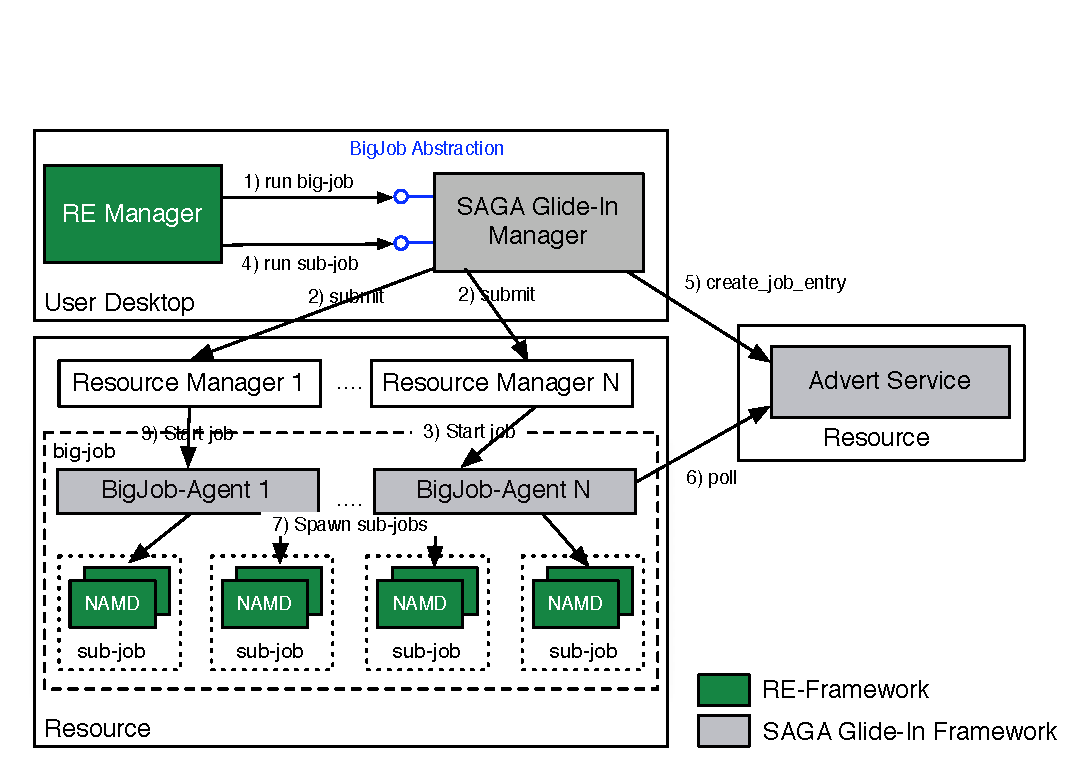
\includegraphics[scale=0.6]{figures/Bigjob_arch.pdf}
% \caption{\small SAGA/BigJob Architecture}
% \label{fig:centralized}
% %\vspace{-1em}
% \end{figure}


In the centralized version (Figure~\ref{fig:async}(a)) of the asynchronous replica exchange (Case II), the master launches and monitors the replicas. As and when it finds a replica in done state, the master starts searching for an appropriate partner from any other replicas in done state. The decision as to make the exchange or not is made using the Metropolis scheme.  %Whether or not a successful exchange takes
%place, the master again monitors all the replicas and repeats the
%steps mentioned.
After each successful exchange the master re-launches the replicas involved in the exchange and continues to monitor the replicas.

\subsubsection{Decentralized Asynchronous RE}


%%%%% FIGURE %%%%%
\begin{figure}
\centering
\subfigure[Control Flow: Centralized Replica Exchange]{
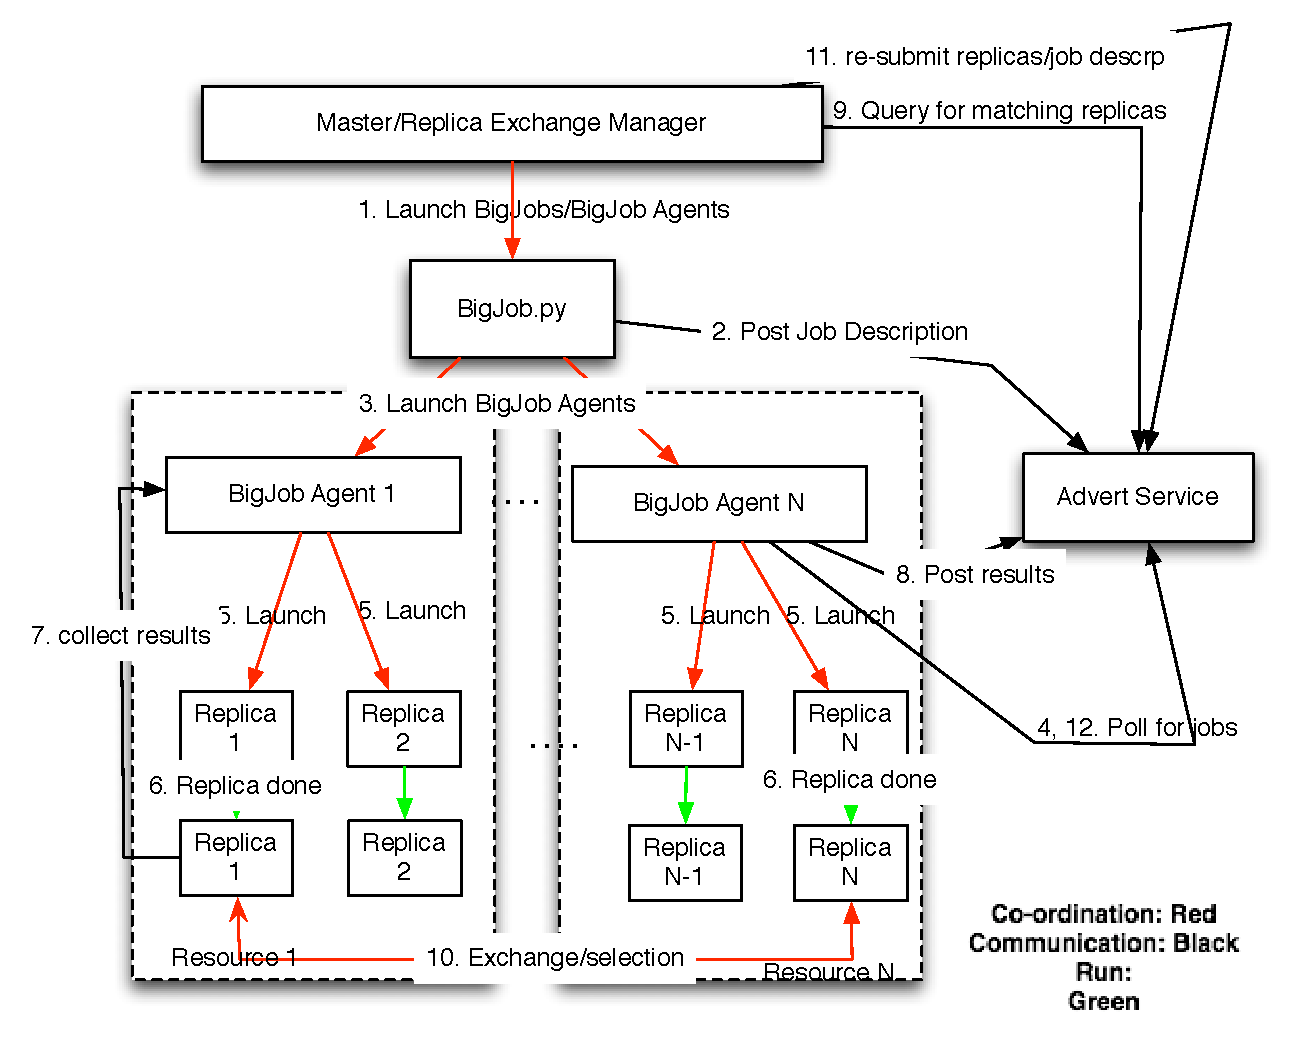
\includegraphics[width=0.46\textwidth]{figures/cent_control.pdf}
%\label{fig:async:b}
}
\subfigure[Control Flow: Decentralized Replica Exchange]{
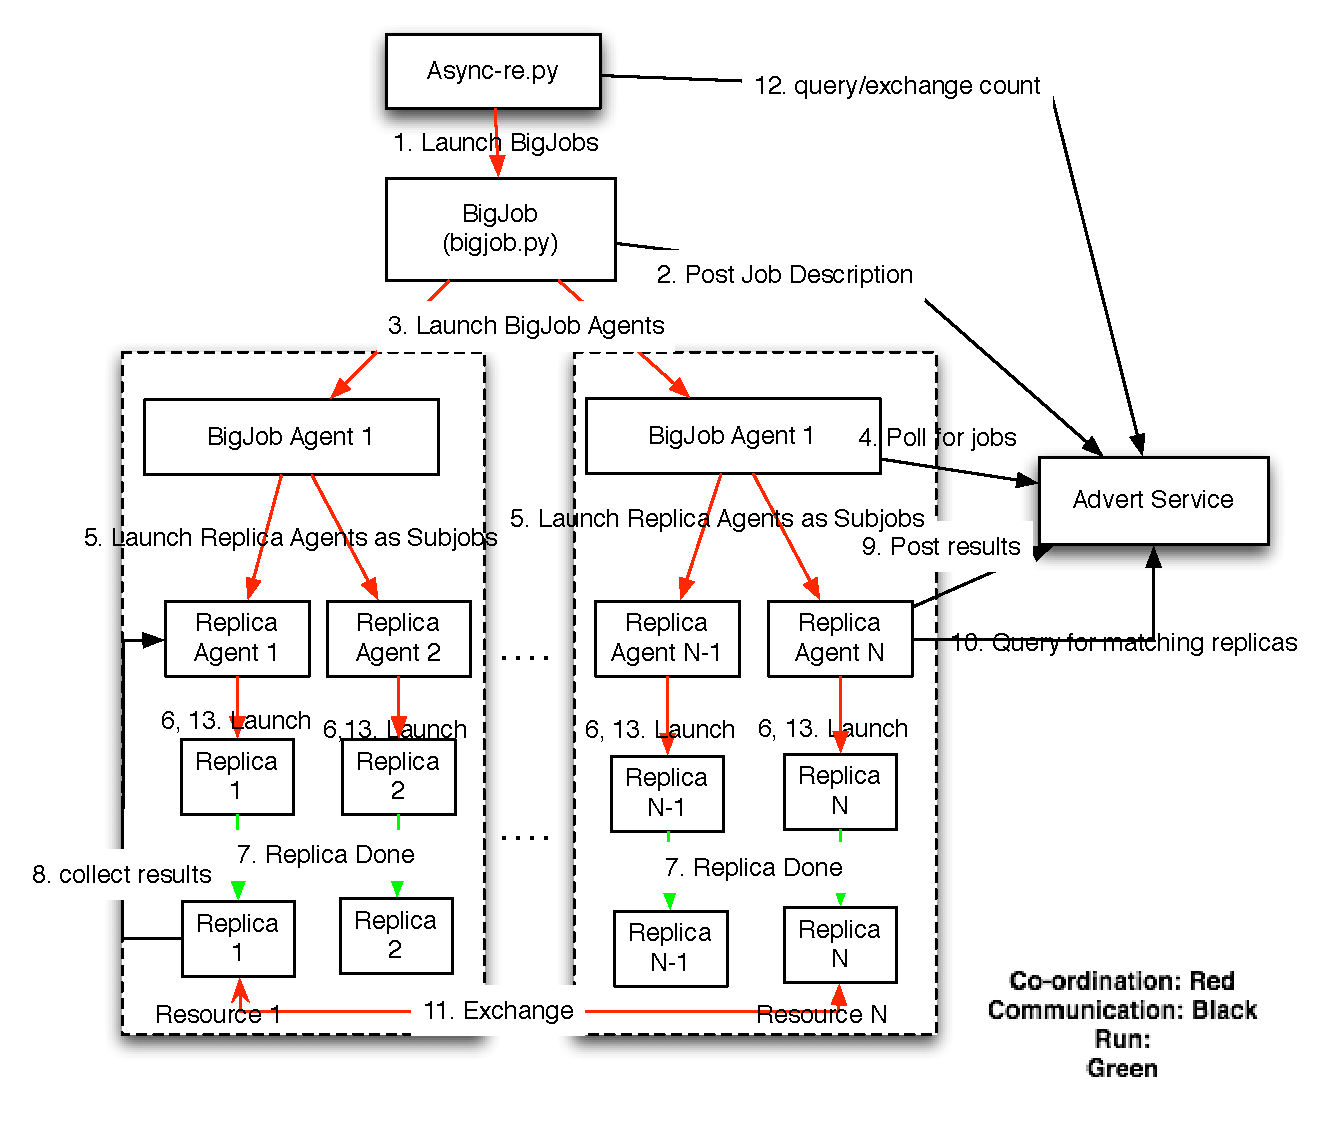
\includegraphics[width=0.46\textwidth]{figures/dec_control.pdf}
%\label{fig:async:b}
}
% 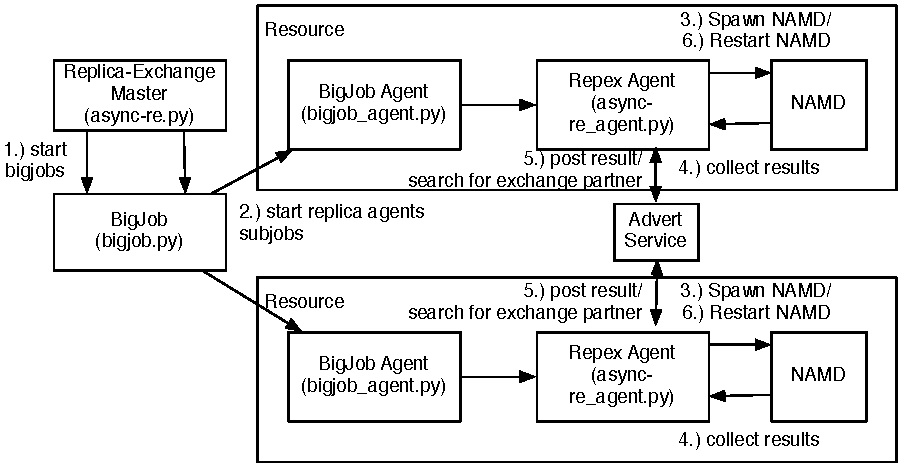
\includegraphics[scale=0.50]{figures/decentralized_architecture.pdf}
\caption{\small In the centralized asynchronous RE (Figure 1(a))all the replicas are managed by the master, where as in the decentralized asynchronous RE version(Figure 1(b)), for each replica there is a replica agent which individually manages the replica.}
\label{fig:async}
%\vspace{-1em}
\end{figure}
%%%%% FIGURE %%%%%

%
%%%%% FIGURE %%%%%
\begin{figure}
\centering
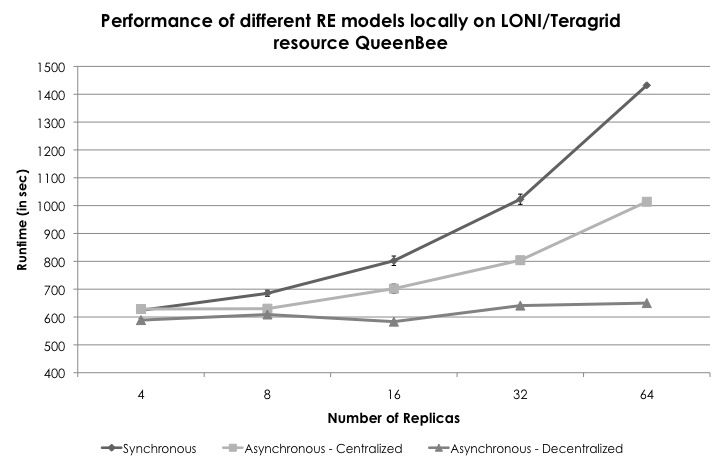
\includegraphics[scale=0.30]{data/1BJ_comparison.jpg}
\caption{\small The graph shows the mean run times of synchronous and asynchronous - centralized and decentralized RE simulations. Each experiment has been repeated at least 10 times.}
\label{fig:graph}
\vspace{-1em}
\end{figure}

 
\alnote{we should write Case consistently with small or capital letter}
In the decentralized version (Case III) version
(Figure~\ref{fig:async}(b)), an agent is launched for each replica. %The agent is nothing but a wrapper
%script for the replica. 
The agent then runs and monitors the replica and looks for partners to exchange when appropriate. In this case, the agent carries out the various tasks needed to conduct the exchange. %The temperatures,
%energies and states of a replica are reported to and retrieved from
%the SAGA advert service. 

Although both Case II and Case III implement the asynchronous 
RE algorithm, they differ subtly. The replicas
are either managed by a master (Case II) or each replica
is managed individually (Case III). We propose Case III so as to not let the centralized master become a bottleneck, which can happen very quickly with a large number of replicas.
% We have to bear in mind that while Case II and Case III both implement the same asynchronous RE algorithm, they do it differently.
% At first glance it appears to be a question of philosophy, whether to
% let the replicas be managed by a master or to let each replica be
% managed individually.
%There could be implications effecting the performance of the
%algorithm. Where as in Case II, the master has to manage all the
%replicas and since it can only manage one replica at a time, although negligible, it is a cause for concern with large number of replicas. %The effect could be negligible and might now effect the overall performance.
%But the decentralized version (Case III) has no
%such issues as each replica is managed individually. % \jhanote{The distinction between Case 3 and 2 needs to
%  be made more clear. The following is ``implementation detail''. What
%  is the conceptual difference between Case 3 and Case 2?}

\section{SAGA BigJob - A Pilot-job Framework}

The Simple API for Grid Applications (SAGA)~\cite{saga_gfd90} is an API standardization effort within the Open Grid Forum (OGF)~\cite{ogf_web}, an international standards development body concerned primarily with standards for distributed computing. The various tasks that are carried out using the SAGA APIs include file staging, job spawning and the conduction of the exchange attempts.

Previously, we demonstrated the usage of the SAGA Pilot-Job framework~\cite{saga_bigjob_condor_cloud} -- called the BigJob, to run RE simulations across multiple, heterogeneous, distributed Grid and Cloud infrastructures~\cite{Luckow:2008fp}. Here we are using the SAGA BigJob to efficiently request and manage computational resources. 


\section{Comparison of different algorithms}

%While the traditional RE limits the exchanges to only neighboring temperatures, an asynchronous RE does not. This is not a concern when the number of replicas is small and there is little chance of an exchange between non-adjacent temperatures. However, as the number of replicas increases, the difference between the target temperatures becomes small enough to allow exchanges between non-adjacent temperatures. This also allows for 'crosswalks' to happen. The larger the number of crosswalks, the better is the performance of the simulation.

%To evaluate the performance of the various models of RE we have discussed in the abstract, we conducted several experiments on Teragrid and LONI resources. 
%In the following sentences we will analyze the performance of synchronous RE(Case I) with centralized asynchronous RE(Case II). 

\subsection{One machine/one BigJob}
We configured the Cases I, II \& III to run parallel NAMD simulations with 4, 8, 16, 32 and 64 replicas sampling a temperature between 300 and 1000 K. One BigJob is launched with sufficient cores while each replica uses 16 MPI processes and runs 500 time steps between exchange attempts. The metric used is the time to complete 16, 32, 64, 128 and 256 attempted exchanges, respectively. It should be noted that the ratio between the number of replicas and the number of attempted exchanges is kept constant, for the purpose of comparison.  %Both cases were run over 1, 2 and 4 machines, where the BigJobs are distributed equally across the resources. 

%The experiments could be potentially run across an infinite number of dissimilar machines.  
%The initial results suggest that the performance has improved at two levels: (i) the time to completion of Case II is reduced by over 200\% compared to Case I and (ii) there is considerable reduction in the time to completion when running across four machines instead of only 1 machine, by as much as 65\%.

The mean run time is obtained by subtracting the queue wait time of the BigJob from the total time. To understand the performance gains(Figure~\ref{fig:graph}) we need to understand the logic behind synchronous and asynchronous RE and how it inevitably influences the implementation. As the ratio between the number of replicas and number of exchanges is kept constant, ideally, the runtime must remain constant too. But, in Case I, the master alone manages the whole simulation. And when it needs to make the exchanges and re-launch large number of replicas after the exchange step, it becomes a bottleneck.. In Case II, the master only has to re-launch two replicas at any one exchange and scales better than Case I. In Case III, each replica has its own manager and this eliminates the delays caused by a central master. This is the difference that we see in the graph. 


%
%%%%% FIGURE %%%%%
\begin{figure}
\centering
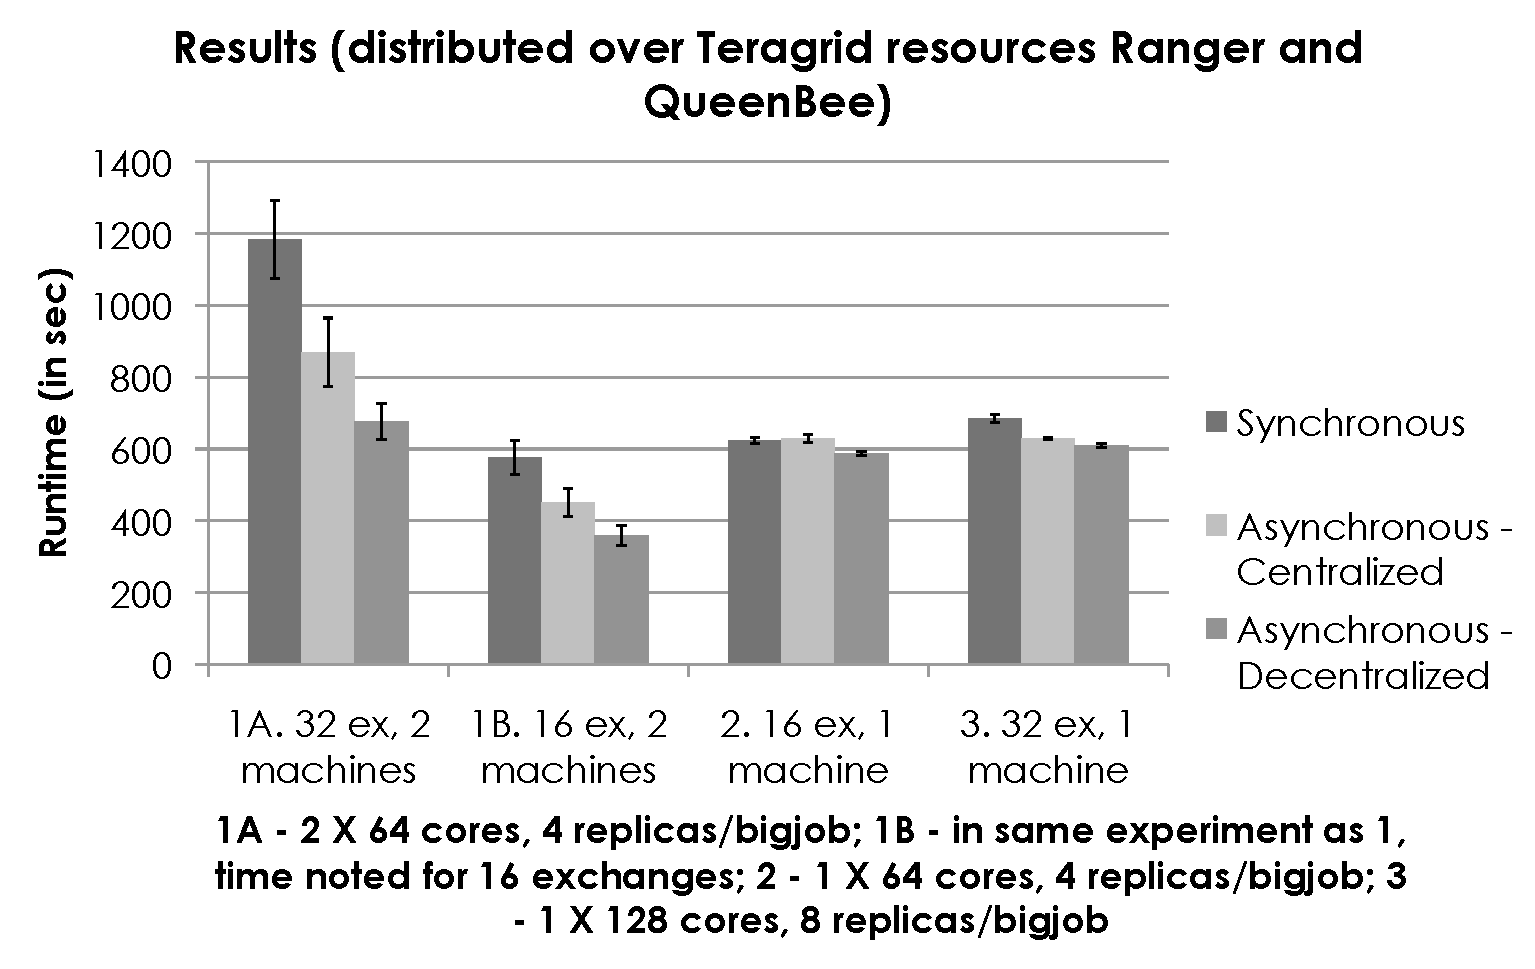
\includegraphics[scale=0.30]{data/2BJ_comparison.pdf}
\caption{\small The graph shows the mean run times of synchronous and asynchronous - centralized and decentralized RE simulations. Each experiment has been repeated at least 10 times.}
\label{fig:graph2}
\vspace{-1em}
\end{figure}

\subsection{Two machines/two BigJobs}

We chose two Teragrid machines - Ranger and QueenBee to run Cases I, II \& III. In each case, 2 BigJobs are launched on each machine. And, 4 replicas are assigned to each BigJob, and 32 exchanges are attempted. In the distributed runs, the run time starts when any one of the BigJobs becomes active. The second BigJob may or may not become active before the simulation ends. 

From the graph, it can be seen from the graph that the distributed runs take longer than the local run. There are two reasons:
(i) The co-ordination and communication across two machines takes longer
(ii) The waiting time of the second machine.

Comparing 1B and 2 in graph, it also should be observed that it is beneficial to request more cores for more machines and use more replicas to make more exchanges.
\athotanote{do we need a graph showing performance in the best case scenario?}In the best case scenario, where both the BigJobs on 2 different machines start instantaneously upon submission, Cases II and III almost equal their respective performances on a single machine. But Case I underperforms and one of the reasons is the heterogeneous infrastructure (QueenBee and Ranger have different processing powers). At each exchange step, all the replicas will have to wait for the replicas running on the slower machine. Also, since all the exchanges are carried out after the synchronization, the time to stage the configuration files to all the replicas (across two machines) keeps going up with more replicas.

In Case II, as the exchanges are done in an asynchronous manner, the slower machine does not noticeably effect the overall performance. Due to the same reason, the effect of  the additional time it takes to stage configuration files across two machines is not readily noticeable. 

In Case III, again, the exchanges are done in an asynchronous manner and effect of the slower replicas is negligible. And, there is no staging of configuration files, as the temperatures are exchanged via the advert service. Hence, Case III is most suited for distributed experiments. 

\subsection{More than two machines}

After conducting the experiments over one and two machines, we are in a position to predict the performance of the different RE algorithms over more than two machines. 
There is no question as to whether the performance of Case I degrades or not. It certainly does across two machines and certainly will across three or four machines due to the same reasons specified above. The question is whether Case II and more importantly Case III perform at the same level across more than two machines. 

In Case II, when the two BigJobs start at different times, the replicas running under particular BigJob start and end at the same time and thus make exchanges - making the exchanges with replicas on the same machine. When the BigJobs start almost simultaneously, all the replicas become available to make exchanges about the same time. In this case, there is greater chance of exchanges happening across different machines. Therefor, the performance of Case II, when running across more than two machines, might fluctuate. But, its performance is going to be close the performance of Case II over two machines. 

In Case III, there is no staging of configuration files involved and hence the performance is going to be similar to Case III over two machines. 


%In Case I, the pair-wise replica exchange can occur only between replicas of the same generation. Therefore, each exchange step is attempted only after all the replicas have finished running. After the exchange, all the replicas are restarted sequentially. This inserts a delay between the start time of the first replica, the last replica and the replicas in between. %As more resources become available at different times, the replicas already running or done are forced to wait for the newly running replicas to finish before moving on to the next exchange step. %Each exchange step is counted as an exchange.
%In Case II, the pair-wise replica exchange can take place between any two replicas in the ensemble irrespective of generation. As more resources become available, the new replicas join the ensemble immediately and the replicas already running are not restrained from attempting exchanges or restarting. This gives the asynchronous or synchronous RE a slight advantage. But with a large number of replicas we could easily see large difference.
%\athotanote{Further, we show performance gains by running across more than one machine. By running across more than one machine, we demonstrate the ability to divide the jobs into smaller sub-jobs and then distribute them across a number of machines, thereby reducing the risk of long queue wait times on an over-crowded resource. In Figure~\ref{fig:graph}, it can be seen that the asynchronous RE time to completion improves almost by a factor of 3 when moving from one machine to four machines. This was caused due to the fact that when the experiment was done on one machine, by the time the experiment ended, only 64 cores were allocated by the resource manager. But on the other hand, when the experiment was launched across four machines, it received an allocation of 64 cores on each of the four resources. The improvement that is seen in the case of synchronous RE from one to four machines is also due to a similar reason.} %The asynchronous RE appears faster by a couple of minutes due to the fact that when the BigJobs become available randomly, the synchronous RE has to wait for the newly running replicas to finish.

%slightly over 2 machines, but again increases over 4 machines. This is due to the fact that the experiments have been run only a handful of times but, over time, it can be assumed that it will result in reduced queue wait times.

\section{Conclusion}



%\athotanote{is this right? }
% We are also going to have a wider group of replicas to look at for
% each replica as we are not pairing the replicas.

% Also, we have the usual advantages of using a pilot-job,
% such as reduced queue wait times by not having to submit to the queue
% at every step.  We also provide major advantages when compared to
% Parashar et al.

%  to run the asynchronous RE simulations,
% including the ability to run MPI
% jobs.
% ??We need to evaluate the performance of our models and compare with other models for conducting replica exchange simulations.


%%%%% FIGURE %%%%%
%\begin{figure}
%\centering
%\subfigure[Time to complete 64 exchanges on QB with two 64 core BigJobs and on both QB/Louie jointly with a 64 core BigJob on each machine.]{
%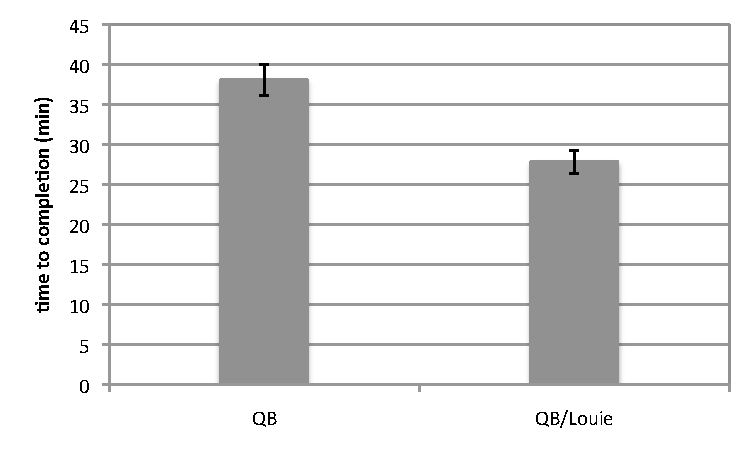
\includegraphics[width=0.40\textwidth]{figures/graph1.pdf}
%\label{fig:subfig3}
%}
%\hspace{0.5cm}
%\subfigure[Time to complete different number of exchanges on QB/Louie with a 64 core BigJob on each machine.]{
%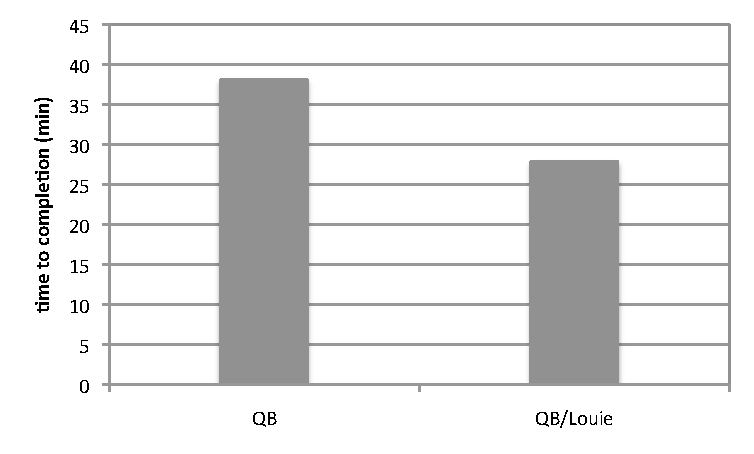
\includegraphics[width=0.40\textwidth]{figures/graph2.pdf}
%\label{fig:subfig4}
%}
%\caption{\small In Figure 2(a), we can see the improvement in performance when run on more than one machine. It is due to the fact that usually the first queued job becomes active before the second on a machine and running jobs on more than one machine solves this problem. In Figure 2(b), we can see consistent performance over prolonged runs, making 32, 64 and 128 exchanges.}
%\label{fig:graphs}
%\vspace{-1em}
%\end{figure}
%%%%% FIGURE %%%%%

An important motivation for this work is to implement a scheme that does not depend on a
static, well defined model of resource availability. %We test and scale
%our implementation on production level grids such as Teragrid and
%LONI~\cite{LONI_web}.
Preliminary results, shown in Figure~\ref{fig:graph}, indicate the most important advantages of asynchronous RE and SAGA/BigJob over traditional RE: (a) allows for exchanges to occur between replicas with non-nearest temperatures, which in turn allows crosswalks to happen (b) a reduced time to completion when running on more than one machine due to improved resource availabilities, (c) the advantage of using a pilot-job mechanism, which eliminates the waiting times at the local resource manager, and (d) the ability to scale out across different production level infrastructure, such as, the Teragrid and LONI.
% It performs well even after doubling and quadrupling the number of
% exchanges required to complete the simulation. The time to
% completion only increases by 35\% after doubling and 117\% after
% quadrupling the number of exchanges.
%\athotanote{should the results
%  be included in the conclusion or in a separate results section? Do
%  you agree with the \# of exchanges scheme to show the data?}
% Unfortunately we have results only for Case II currently, but 

%In summary, we have established the ability to scale-out across different
%infrastructure and compared the performance of the asynchronous
%RE with the synchronous RE at large scales. 
Further, we compare the traditional RE model(Case I) and the centralized(Case II) and decentralized(Case III) models of the asynchronous replica exchange by modeling and repeating the experiments a reasonable number of times, so as to accurately quantify the scientific and performance gains. %We also propose to measure the frequency with which crosswalks occur with increasing number of replicas and measure the advantages due to a decentralized implementation in the full paper.


%With this asynchronous replica exchange mechanism we can improve the
%number of exchanges per unit time, a key parameter in judging the
%performance of a replica-exchange mechanism. \athotanote{is this
 % right? }  We are also going to have a wider group of replicas to
%look at for each replica as we are not pairing the replicas. Also, we
%have the usual advantages of using a pilot-job, such as reduced queue
%wait times by not having to submit to the queue.  Unfortunately we
%dont have results \jhanote{What results can we present -- any? some?},
%so we will say, (i) we establish the ability to scale-out (distributed
%and exa-scale) across different infrastructure (ii) compare the Async
%versus sync formulation at unprecedented scales \jhanote{At least
%  outline what infrastructure we / you are planning to use?} (iii)
%compare different implementations of the Async version
 
 \bibliographystyle{IEEEtran} 
 \bibliography{literature,saga}


\end{document}

